% Created 2022-01-17 Mon 08:14
% Intended LaTeX compiler: pdflatex
\documentclass[presentation]{beamer}
\usepackage[utf8]{inputenc}
\usepackage[T1]{fontenc}
\usepackage{graphicx}
\usepackage{longtable}
\usepackage{wrapfig}
\usepackage{rotating}
\usepackage[normalem]{ulem}
\usepackage{amsmath}
\usepackage{amssymb}
\usepackage{capt-of}
\usepackage{hyperref}
\usepackage{color}
\usepackage{listings}
\usepackage{color}
\usepackage{listings}
\DeclareTextFontCommand{\texttt}{\color{blue}\ttfamily}
\usetheme{default}
\author{Maikol Solís}
\date{2022-01-17}
\title{Emacs workshop 2022: Day 1}
\AtBeginSection[]{\begin{frame}[plain]\frametitle{}\tableofcontents[currentsection]\end{frame}}
\hypersetup{
 pdfauthor={Maikol Solís},
 pdftitle={Emacs workshop 2022: Day 1},
 pdfkeywords={},
 pdfsubject={},
 pdfcreator={Emacs 27.2 (Org mode 9.6)}, 
 pdflang={English}}
\usepackage{biblatex}

\begin{document}

\begin{frame}[plain]
    \maketitle
\end{frame}

\begin{frame}[plain]
    \tableofcontents
\end{frame}



\section{About me}
\label{sec:org60eb3c6}

\begin{frame}[label={sec:org681765f}]{}
\begin{itemize}
\item Maikol Solís, Ph.D
\item Professor Escuela de Matemática, UCR
\item Researcher at CIMPA
\end{itemize}
\begin{center}

\includegraphics[width=100]{foto.png}
\end{center}
\end{frame}

\begin{frame}[label={sec:org48afd10},fragile]{My own journey}
 \alert{\alert{Needs:}} \LaTeX{}, R, email, organization tools, tracking papers, writing.


\begin{itemize}
\item\relax [2002-2015] Pen and paper (still), Word/OpenOffice, TeXstudio/Texmaker, Lyx, gmail/google calendar (still), apps for tasks, Sublime editor, Rstudio (still), and so on.
\item\relax [2016-2017] I started using spacemacs, but I couldn't understand it.
\item\relax [2017] I tried using vim/neovim, but still I was lost.
\item\relax [2018-2020] I discovered VSCode (and like it!). But the ecosystem was too restrictive.
\item\relax [2020-\(\infty\)] In 2020, I learned about \texttt{org-mode} and \texttt{org-roam}.  I restart using Emacs with Doom-emacs.
\end{itemize}

Little by little I have all my workflow in Emacs now.
\end{frame}


\section{About (GNU) Emacs}
\label{sec:org07f6d9f}

\begin{frame}[label={sec:org6bf3dba}]{What is Emacs?}
\begin{itemize}
\item Free/Libre text editor.
\item Extensible and customizable (\(\to\infty\)).
\item A platform for text-related applications.
\end{itemize}
\end{frame}

\begin{frame}[label={sec:org2f0bdd6},fragile]{Emacs History}
 \begin{description}
\item[{1976}] Richard M. Stallman wrote the first Emacs (“Editor MACroS”).
\item[{1984}] RMS started with the GNU Emacs (free opensource) in Lisp and C.
\item[{1985}] Release of first Emacs version (13.0) only supporting console.
\item[{2001}] GNU Emacs has graphical interfaces (an other modern features).
\item[{2003}] Carten Dominik creates \texttt{org-mode} as an independent package.
\item[{2006}] \texttt{org-mode} is included by default in Emacs.
\item[{Present}] New features like \texttt{org-babel}, programming languages, JSON, native-compilation, SQLite, PGTK, etc.
\end{description}
\end{frame}

\begin{frame}[label={sec:orgeda3a9d},fragile]{Emacs features}
 \begin{itemize}
\item Content aware editing mode.
\item Uses Emacs Lisp dialect (functional programming language).
\item Highly customizable.
\item Has +10,000 built-in commands and macros to create new-ones.
\item Full Unicode support.
\item Real-time display editor.
\item Multiple functions: Project planner, Calendar, Debugger, Mail reader, a more\ldots{}
\item Exports \texttt{org} files to html, pdf, odt, \ldots{}
\end{itemize}
\end{frame}

\begin{frame}[label={sec:org8aca31f}]{Emacs philosophy}
\begin{itemize}
\item The users have all the control in the editor.
\item They can add, remove or modify any feature (no limits).
\item Emacs doesn't care for ``looking'' modern or have a check-box for any option.
\item The user decides how to behave or look the editor.
\end{itemize}


\begin{description}
\item[{The disadvantage:}] \emph{The users NEED TO configure the editor.}
\item[{The big advantage:}] \emph{The users CAN configure the editor.}
\end{description}
\end{frame}


\begin{frame}[label={sec:org80a685c}]{It's a whole journey, so relax.}
\begin{center}

\includegraphics[width=\textwidth]{./road.png}
\end{center}
\end{frame}



\section{About the configuration}
\label{sec:org759eaef}

\begin{frame}[label={sec:org9c8f5e9}]{Let's draw a house}
Imagine someone asks to draw a house like this
\begin{center}
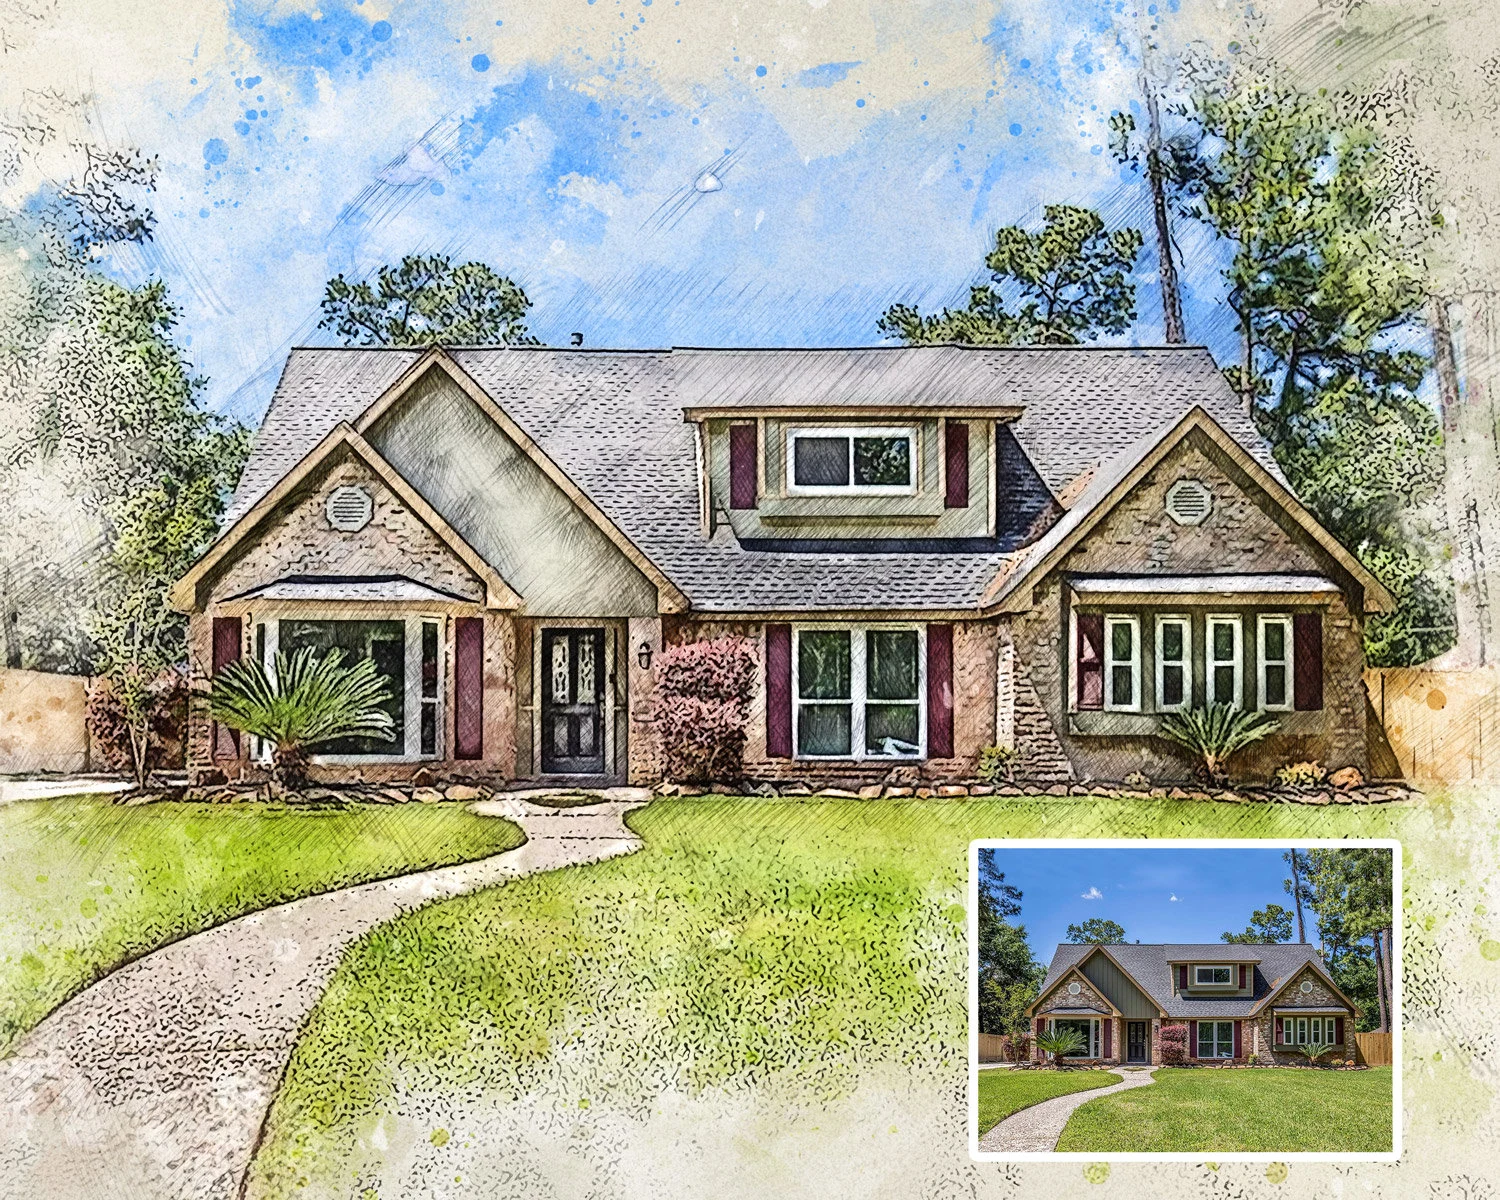
\includegraphics[width=0.5\textwidth]{./house_model.png}
\end{center}

You can do it in different ways\ldots{}
\end{frame}

\begin{frame}[label={sec:orge920835}]{Vanilla Emacs}
\begin{itemize}
\item Nothing is configured yet.
\item Steep learning curve.
\item Default and cleanest configuration of Emacs.
\item Definitely not for beginners.
\end{itemize}

\begin{center}

\includegraphics[height=10em]{./emacs.png}

\includegraphics[height=10em]{./paper.png}
\end{center}
\end{frame}

\begin{frame}[label={sec:orgb7b696b}]{Doom-emacs}
\begin{itemize}
\item With some options preconfigured, but everything can be changed
\item Some learning curve.
\item Thinner, lighter, opinionated.
\item Could be difficult to beginners.
\end{itemize}

\begin{center}

\includegraphics[width=13em]{doom.png}

\includegraphics[width=13em]{pencils.png}
\end{center}
\end{frame}


\begin{frame}[label={sec:org2adc6fa}]{Spacemacs}
\begin{itemize}
\item Almost all is preconfigured and behind abstract layers. However, configuration is possible.
\item Easy learning curve.
\item Fast, Mnemonic, consistent.
\item Beginner friendly.
\end{itemize}


\begin{center}

\includegraphics[height=10em]{spacemacs.png}

\includegraphics[height=10em]{kids.png}
\end{center}
\end{frame}

\section{Doom-emacs}
\label{sec:orgdcc6b6a}
\begin{frame}[label={sec:orga81813b}]{Why chosing doom-emacs?}
\begin{itemize}
\item Doom-emacs is near to vanilla, but with useful preconfigured packages.
\item As user you will need the freedom to configure Emacs.
\item I have found most of the internet help is written for vanilla Emacs or doom.
\item Doom-emacs is a configuration framework rather than started kit.
\end{itemize}
\end{frame}

\begin{frame}[label={sec:orgcb1a286}]{Requirements for the workshop}
\begin{itemize}
\item Emacs 27.2
\item Git 2.23+
\item ripgrep 11.0+
\item GNU Find
\item fd 7.3.0+ (fd-find)
\end{itemize}

Check how to install those packages in your operative system.
\end{frame}

\begin{frame}[label={sec:orge847348},fragile]{Doom-emacs install}
 In console

\begin{verbatim}
git clone https://github.com/hlissner/doom-emacs ~/.emacs.d
~/.emacs.d/bin/doom install
\end{verbatim}

After

\begin{verbatim}
doom doctor
\end{verbatim}
\end{frame}
\begin{frame}[label={sec:orga4af7b0},fragile]{Doom-emacs main commands}
 \begin{itemize}
\item \texttt{doom sync}: Sync the doom configuration.
\item \texttt{doom upgrade}: Update doom and all the packages.
\end{itemize}
\end{frame}


\begin{frame}[label={sec:org26b4cf8},fragile]{Doom-emacs files}
 All the files are in \texttt{\textasciitilde{}/.doom.d/}

\begin{itemize}
\item \texttt{config.el}: Custom configurations.
\begin{itemize}
\item \texttt{(use-package! a-package body)}

Execute body for \texttt{a-package}.
\item \texttt{(after! a-package body)}

Execute body after load \texttt{a-package}.
\item \texttt{(setq variable value)}

Set a variable to a value.
\end{itemize}

\item \texttt{init.el}: Activate/Deactivate modules.
\item \texttt{package.el} Add new packages with \texttt{(package!)}.
\end{itemize}
\end{frame}


\begin{frame}[label={sec:orgc11cd65}]{Where to get help?}
\begin{itemize}
\item \url{https://emacsdocs.org/}
\item \url{https://discourse.doomemacs.org/t/other-learning-resources/48}
\end{itemize}
\end{frame}

\section{Basic operations}
\label{sec:orgc0379df}
\begin{frame}[label={sec:org34c637c},fragile]{Some definitions}
 \begin{description}
\item[{\texttt{SPC}}] Space.
\item[{\texttt{RET} }] Enter.
\item[{\texttt{C-c} }] Press \texttt{Control} + \texttt{c}.
\item[{\texttt{M-x} }] Press \texttt{Meta} (\texttt{Alt}) + \texttt{x}.
\item[{\texttt{C-S-a} }] Press \texttt{Control} + \texttt{Shift} + \texttt{a}.
\end{description}
\end{frame}

\begin{frame}[label={sec:org7fe7db1}]{Buffers, windows and frames}
\begin{center}
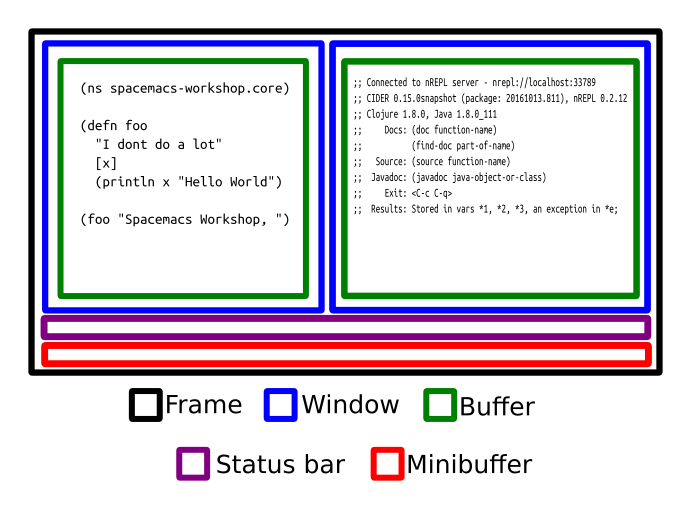
\includegraphics[width=\textwidth]{./frames.png}
\end{center}
\end{frame}

\begin{frame}[label={sec:org380978c},fragile]{Avoiding RSI}
 \begin{itemize}
\item Default shortcuts in vanilla Emacs starts with \texttt{Control} or \texttt{Meta}.
\item In doom all basic commands starts with \texttt{SPC}.
\item Doom-emacs uses a modal (and easier) system called \texttt{evil-mode}. (More later!)
\end{itemize}


\begin{center}
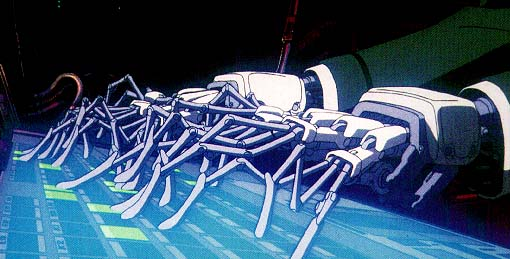
\includegraphics[width=\textwidth]{./ghost.png}
\end{center}
\end{frame}

\begin{frame}[label={sec:orga5e4c0e},fragile]{Basic shortcuts}
 \begin{description}
\item[{\texttt{SPC} }] Display the main menu.
\item[{\texttt{SPC SPC}}] Open a file in project (current folder or git repository).
\item[{\texttt{SPC :}}] \texttt{M-x} execute any command.
\item[{\texttt{SPC h} }] The help system.
\item[{\texttt{SPC h i} }] Official manuals (look for \emph{Org Mode} and \emph{Emacs}).
\item[{\texttt{SPC h d h} }] Doom help.
\item[{\texttt{SPC h d m} }] Doom's module help.
\end{description}
\end{frame}

\begin{frame}[label={sec:org532fe7e},fragile]{Open and saving}
 \begin{description}
\item[{\texttt{SPC f f}}] Opens any file.
\item[{\texttt{SPC f s} o \texttt{SPC b s}}] Save file.
\item[{=SPC f r}] Rename file.
\end{description}
\end{frame}

\begin{frame}[label={sec:orgc800dbc}]{Evil (Extensible VI Layer)}
\begin{center}

\includegraphics[height=3 em]{./evil.png}
\end{center}

\begin{center}

\includegraphics[width=\textwidth]{./vim.png}
\end{center}
\end{frame}


\begin{frame}[label={sec:org62ef4a7},fragile]{Basic evil commands}
 \begin{center}
\begin{tabular}{|cc||cc|}
key & movement & key & action\\
\hline
\texttt{h} & left & \texttt{ESC} & enters normal mode\\
\texttt{l} & right & \texttt{i} & enters insert mode\\
\texttt{j} & down & \texttt{v} & enters visual mode\\
\texttt{k} & up & \texttt{x} & delete char\\
\texttt{0} & start of line & \texttt{x} & delete char\\
\texttt{\$} & end of line & \texttt{r} & replace char\\
 &  & \texttt{u} & undo\\
 &  & \texttt{C-r} & redo\\
\end{tabular}
\end{center}
\end{frame}

\begin{frame}[label={sec:org74e4a45},fragile]{Speaking evil}
 \begin{itemize}
\item \href{https://practical.li/spacemacs/spacemacs-basics/vim-basics.html}{Good tutorial (done for spacemacs)}
\item \href{https://external-preview.redd.it/iigrixvxp5aYN9ox7Gr1dfI\_rhLRotWlLsCafjJqjEQ.png?auto=webp\&s=1594ddc17408cb9186a73c2a6d1a1bf1e00769dd}{Full vim cheat sheet}
\end{itemize}

\begin{block}{Verbs}
\texttt{c} (change), \texttt{d} (delete), \texttt{g} go, \texttt{v} visual (select), \texttt{y} yank (copy)
\end{block}

\begin{block}{Modifiers}
\texttt{\{ \}} beginning/end of paragraph, \texttt{a} around, \texttt{f} find (includes character), \texttt{i} inside, \texttt{s} surround, \texttt{t} till (just before a character)
\end{block}
\begin{block}{Objects}
\texttt{b} block/parentheses, \texttt{p} paragraph, \texttt{s} sentence, \texttt{w} word
\end{block}
\end{frame}
\begin{frame}[label={sec:orgff3b1bb},fragile]{Other evil features}
 \begin{itemize}
\item \texttt{evil-tex}: to handle related \LaTeX{} objects.
\item \texttt{g} and \texttt{z} menus: convient set of utlities.
\end{itemize}
\end{frame}

\section{Let's practice}
\label{sec:orgb346b31}

\begin{frame}[label={sec:org36094d2}]{Preparation}
\begin{itemize}
\item Open the latex file.
\item Enable the latex module.
\item Do the exercises.
\end{itemize}
\end{frame}
\end{document}